% To see package versions
%\listfiles%

\documentclass{article}
\usepackage[utf8]{inputenc}
% for large margins
\usepackage[margin=1in]{geometry}
% for \verb
\usepackage{verbatim}
% for \verb inside lists
\usepackage[Q=yes]{examplep}

% fonts to remove the tilde
\usepackage[T1]{fontenc}
% \usepackage{beramono}

%for units
\usepackage[binary-units=true]{siunitx}

% to format the code
\usepackage[newfloat]{minted}
\usemintedstyle{borland}
% for code captioning
\usepackage{caption}

% for table
\usepackage{multirow}

\newenvironment{code}{\captionsetup{type=listing}}{}
\SetupFloatingEnvironment{listing}{name=Code}


%TODO: CHECK FIGURE ORDERING IF SOME ARE FLOATS!%

% to link to mimic
\usepackage{hyperref}

% to put graphs in
\usepackage{graphicx}
\graphicspath{ {images/} }
\usepackage{subcaption}

% for landscape
\usepackage{pdflscape}


% bibliography
\usepackage[
backend=biber,
style=authoryear,
sorting=ynt
]{biblatex}
\addbibresource{bib.bib}




\title{Benchmarking Parallel Application Performance Across SCD Infrastructure}
\author{Callum Iddon }
\date{March 2017}

\begin{document}


\definecolor{code-bg}{rgb}{0.95,0.95,0.95}
\setminted{bgcolor=code-bg}

\maketitle

\begin{abstract}
Two benchmarks (HPL and IMB) are run across SCARF, LOTUS and the SCD Cloud to measure the effect of bandwidth, latency, distributing cores between nodes and using newer hardware on parallel application performance. A common ranking between different methods of communication is shown in the results of all benchmarks (SHM-1, SHM-2, IBV then TCP). Whilst using newer processors is found to have the greatest impact on parallel application performance, both SCARF and LOTUS are shown to be able to perform as effectively between cores on separate hosts as on an individual host - despite lower bandwidth and higher latency. The Cloud performs similarly to the oldest SCARF host (scarf10) but with a higher TCP bandwidth.
\end{abstract}


\tableofcontents

\section{Introduction}

    \subsection{Background}
        \paragraph{}
        The Scientific Computing Department (SCD) provides a number of compute resources. Across the different infrastructures, the varying CPUs, interconnect bandwidth and latencies have an unquantified effect on parallel applications. Also unmeasured is the effect of choices within each service, such as using newer hardware or distributing cores between nodes.

    \subsection{In This Project}
        \paragraph{}
        Comparison metrics are gathered for parallel application performance across three SCD services - SCARF, LOTUS and the SCD Cloud. The aim is to provide results that can inform deployment decisions for parallel applications using the Message Passing Interface (MPI) libraries going forward.

        \paragraph{}
        Two specific metrics are recorded - bandwidth and latency - using the IMB PingPong benchmark. Application performance is then measured more generally according to the results from the HPL TOP500 test. On SCARF and LOTUS, these are taken on cores on the same node, spanning different nodes, and on different hardware versions. On the Cloud, they are taken from one VM and across two VMs (on different hypervisors).

    \subsection{Report Layout}
        \paragraph{}
        This report starts by introducing the benchmarks and explaining how they were set up. Detailed methods for running them are set out to allow reproducibility. The results are analysed, first to explain small adaptions to the method and then for comparison between different options. In the appendices, there are example outputs from each of the benchmarks and the data in tabulated form.

\section{Methods}

    \subsection{Overview}
    \label{overview-of-methods}
    There are two benchmarking applications to run on each system.

    \begin{description}
        \item[IMB PingPong] uses MPI to send messages of increasing size both ways between two processes [\cite{intel2016}]. Latency is the average time for the message of zero size to cross one way between the two processes. Bandwidth is the throughput at different message sizes. The only dependency to run this benchmark is an MPI library.
        \item[HPL TOP500] solves a large matrix problem over distributed compute and memory resources [\cite{hpl2016}]. The time taken to solve the problem gives a measure of parallel application performance in FLOPS (floating point operations per second). The software relies on a linear algebra library as well as an MPI library.
    \end{description}

    \paragraph{}
    For all infrastructures, running a benchmark between cores on the same host is referred to as shared host memory (SHM). Running a job between hosts is normally over Ethernet connection (TCP) but on SCARF there is the additional option of running over Infiniband (IBV). In general benchmarks are repeated five times for each setup to ensure that there is some consistency amongst results. On the Cloud, there is no exclusive option so other users' activity on the hypervisors can only be accounted for by averaging over more repeats (30).

    \subsection{Installation} \label{installation}

        \paragraph{}
        On the Cloud, the benchmarks need to be installed from scratch, alongside any dependencies. On SCARF and LOTUS, the MPI and linear algebra libraries are pre installed alongside HPL but IMB must be compiled from source and linked to the existing MPI libraries.

        \subsubsection{Cloud} \label{cloud-installation}

        \paragraph{}
        An SL6 no GUI virtual machine was used. The MPI library was OpenMPI and the linear algebra library was OpenBLAS (both from yum). A makefile was created to link to these libraries (Appendix \ref{appendix:makefile}).

            \begin{code}
            \captionof{listing}{Installing IMB and HPL on a Cloud VM}
            \label{code:builds-cloud-build-sh}
            \begin{minted}{bash}
# Install IMB PingPong
sudo yum -y install openmpi-devel  # install OpenMPI
wget https://software.intel.com/sites/default/files/managed/a3/53/IMB_2017.tgz
tar -xvf IMB_2017.tgz
source /etc/profile.d/modules.sh   # enable environment-modules
module load openmpi-1.10-x86_64    # load the MPI module
cd imb/imb/src
make CC=mpicc                      # compile
cd -

# Install HPL
wget http://www.netlib.org/benchmark/hpl/hpl-2.2.tar.gz
tar -xvf hpl-2.2.tar.gz
sudo yum -y install openblas-devel openblas-static # install OpenBLAS
cd hpl-2.2/
# Copy in the makefile from the appendix now.
make arch=Linux_SL6_Intel64                        # compile
            \end{minted}
            \end{code}


        To run MPI between VMs on the Cloud (without a scheduler), SSH keys must be set up. There is no need for encryption provided the keys never leave either machine.
            \begin{code}
            \captionof{listing}{Setting up SSH keys between
            Cloud VMs}
            \label{code:builds-cloud-setupssh-sh}
            \begin{minted}{bash}
# On both VMs
sudo chown $USER:root ~/.ssh # Cloud VMs start with root:root, allow yourself access

# On one
ssh-keygen -t rsa # create key pair
cat ~/.ssh/id_rsa.pub >> ~/.ssh/authorized_keys # allow access to key
scp ~/.ssh/* <other VM hostname>:~/.ssh/ # copy this setup to the other machine
            \end{minted}
            \end{code}

        \subsubsection{SCARF and LOTUS}
        On both LOTUS and SCARF, the IMB benchmark was compiled from source.

            \begin{code}
            \captionof{listing}{Installing IMB on SCARF and LOTUS}
            \label{code:builds-jasmin_scarf-buildimb-sh}
            \begin{minted}{bash}
# Install IMB PingPong
wget https://software.intel.com/sites/default/files/managed/a3/53/IMB_2017.tgz
tar -xvf IMB_2017.tgz
cd imb/imb/src
gmake CC=mpicc
            \end{minted}
            \end{code}


        On LOTUS, the HPL binary is located at \verb|/apps/src/hpl/hpl-2.2/bin/Linux_Intel64/xhpl| which is installed using the Intel MKL and Platform MPI libraries.

        On SCARF, HPL is optimised for each processor at \verb|/apps/procspec/hpl/2.2/bin/Linux_Intel64/xhpl|, to avoid this advantage, the scarf10 (least optimised) version was used for all processors by copying this binary to a shared location between processors (see section \ref{running-HPL-SCARF}).




    \subsection{Running IMB}

        \paragraph{}
        In general, the benchmarks are submitted by shell scripts that take care of configuration parameters, platform specific parameters (eg LSF flags) and running repeats of the benchmarks. On the systems where there is a job scheduler (LOTUS and SCARF), these scripts submit the jobs where the benchmarks are actually run. On the Cloud, a cronjob is setup to run the script at regular intervals.

        \subsubsection{Configuration}

        \paragraph{}
        IMB is configured by command line parameters.

        \begin{description}
            \item[-iter n] ensures that \verb|n| repeats of each message size are taken and averaged. 1000 was chosen because it was the largest number of repeats that maintained a reasonable time to run on the slowest infrastructure (Cloud, between two VMs). It was also the default for smaller message sizes.
            \item[-time t] sets a maximum time \verb|t|(s) for all repeats of a message size. 200 was chosen because it is significantly high such that this maximum was never reached.
            \item[-msglog a:b] sets a minimum and maximum ($2^{a}$, $2^{b}$) for the message sizes.
            \item[-iter\_policy] sets the behaviour with large message sizes and whether to reduce the number of repeats. Given that the number of repeats is feasible, setting this to \verb|off| means that the same number of repeats are tested for each message size.
        \end{description}

        \subsubsection{SCARF}
            \begin{enumerate}
                \item Create a top directory and \verb|cd| into it (e.g. \verb|/home/cseg/scarf565/SCARF_IMB|).
                \item Install IMB inside this directory as in Code \ref{code:builds-cloud-build-sh}. This should create \verb|imb/imb/src/IMB-MPI1|.
                \item Submit jobs to run the benchmark for five repeats across each host group. For each host group, run the benchmark between hosts using TCP, using Infiniband and on the same host. Use Code \ref{code:tests-scarf_imb-runimbscarf-sh} from inside the top directory.
                    \begin{code}
                    \begin{minted}[breaklines=true]{bash}
#! /bin/bash
hostgroups=(scarf10 scarf11 scarf12 scarf13 scarf14 scarf15 scarf16)
# Make the outputs directory if it doesn't exist
mkdir -p $PWD/outputs
for specificHost in ${hostgroups[@]}; do # For each hostgroup
    for perTile in 1 2; do # Span one (2) node or two (1)
        if [ $perTile -eq 1 ]; then
            # If going between nodes, specify different interconnect flags
            pFlagOptions=(-TCP -IBV)
        else
            # If not, there are no interconnect flags
            pFlagOptions=("")
        fi
        for pFlag in "${pFlagOptions[@]}"; do # Step through interconnect flags
            for repeat in 1 2 3 4 5; do # Repeat the benchmark

bsub << %EndOfInput%
#BSUB -x
#BSUB -n 2
#BSUB -R "span[ptile=$perTile]"
#BSUB -J PingPong
#BSUB -o $PWD/outputs/%J.out
#BSUB -e $PWD/outputs/%J.err
#BSUB -W 0:45
#BSUB -m "$specificHost"
mpirun -lsf -prot $pFlag $PWD/imb/imb/src/IMB-MPI1 -iter 1000 -time 200 -msglog 0:24 -iter_policy off PingPong
%EndOfInput%

            done
        done
    done
done
                \end{minted}
                \captionof{listing}{Submitting IMB to SCARF}
                \label{code:tests-scarf_imb-runimbscarf-sh}
                \end{code}
            \end{enumerate}
        \subsubsection{LOTUS}
            The method for running IMB on LOTUS is similar but there is no Infiniband available and there is a different \verb|mpirun| command.

            \begin{enumerate}
                \item Create a top directory and \verb|cd| into it (e.g. \verb|/home/users/ciddon/JASMIN_IMB|).
                \item Install IMB inside this directory as in Code \ref{code:builds-cloud-build-sh}. This should create \verb|imb/imb/src/IMB-MPI1|.
                \item Submit jobs to run the benchmark for 5 repeats across each host group. For each host group, run the benchmark between hosts and within the same host. Use Code \ref{code:tests-jasmin_hpl-runimbjasmin-sh} from inside the top directory.

                    \begin{code}
                    \captionof{listing}{Submitting IMB to LOTUS}
                    \label{code:tests-jasmin_hpl-runimbjasmin-sh}
                    \begin{minted}[breaklines=true]{bash}
#! /bin/bash
hostgroups=(ivybridge512G ivybridge2000G haswell256G ivybridge128G broadwell256G)
# Make the outputs directory if it doesn't exist
mkdir -p $PWD/outputs
for specificHost in ${hostgroups[@]}; do # For each hostgroup
    for perTile in 1 2; do # Span one (2) or two (2) nodes
        for repeat in 1 2 3 4 5; do # Repeat the benchmark

bsub << %EndOfInput%
#BSUB -x
#BSUB -q par-multi
#BSUB -n 2
#BSUB -R "span[ptile=$perTile]"
#BSUB -J PingPong
#BSUB -o $PWD/outputs/%J.out
#BSUB -e $PWD/outputs/%J.err
#BSUB -W 0:45
#BSUB -m "$specificHost"
mpirun.lotus -prot $PWD/imb/imb/src/IMB-MPI1 -iter 1000 -time 200 -msglog 0:24 -iter_policy off PingPong
%EndOfInput%

        done
    done
done
                    \end{minted}
                    \end{code}
            \end{enumerate}
        \subsubsection{Cloud}

            \paragraph{}
            Two virtual machines are required to run IMB. The main VM (where the job is initialised from) must have at least two cores.

            \paragraph{}
            Using \url{http://mimic.gridpp.rl.ac.uk/}, under \verb|Cloud -> Open Nebula|, find the VMs and ensure that they are on different hypervisors (by clicking for more information).

            \begin{enumerate}
                \item Install IMB in the home directory of both VMs and setup SSH as in section \ref{cloud-installation}.
                \item Create a top directory on the main VM eg \verb|/home/tan49775/Cloud_IMB|.
                \item Create a script (Code \ref{code:tests-cloud_imb-runimbcloud-sh}) in this top directory which will run a repeat of the benchmark each time it is called, incrementing a count file to keep track of the number of repeats. The script ensures the benchmark is run 30 times within the same host and then 30 times between the two VMs. Use a different \verb|HOME_DIR|, \verb|START_DIR| and host address.
                    \begin{code}
                    \captionof{listing}{The script to run IMB once on each call over cron}
                    \label{code:tests-cloud_imb-runimbcloud-sh}
                    \begin{minted}[breaklines=true]{bash}
#! /bin/bash

# Enable the module command
source /etc/profile.d/modules.sh
# Use the module command to set the mpi env
module load openmpi-1.10-x86_64

# Set up some variables
REPEATS_FOR_EACH=30
# Set HOME_DIR and START_DIR to the top directory
HOME_DIR=/home/tan49775  # should contain imb/imb/src.. and Cloud_IMB
START_DIR=$HOME_DIR/Cloud_IMB
COUNT=$START_DIR/count

# Make the output directory if needed
mkdir -p $START_DIR/outputs

num=$(date +"%Y%m%d_%H%M%S")
outputFile=$START_DIR/outputs/$num.out
errorFile=$START_DIR/outputs/$num.err

# If the count file does not exist then initialise it
if [ ! -s $COUNT ]; then echo "1" > $COUNT; fi

# If done enough repeats of one host and two hosts then exit
if [ $(cat $COUNT) -gt $((2 * $REPEATS_FOR_EACH)) ]; then exit 0; fi

# If done enough repeats for one host then use two hosts
if [ $(cat $COUNT) -gt $REPEATS_FOR_EACH ]; then
    echo "#HOSTS=2" > $outputFile
    # Edit the two host addresses here as necessary
    multiHostFlags="--prefix /usr/lib64/openmpi-1.10/ --map-by node  --rank-by node --host vm275.nubes.stfc.ac.uk,vm15.nubes.stfc.ac.uk"
else # Otherwise only use this host
    echo "#HOSTS=1" > $outputFile
    multiHostFlags=""
fi

# Run the benchmark
mpirun -np 2 $multiHostFlags $HOME_DIR/imb/imb/src/IMB-MPI1 -iter 1000 -msglog 0:24 -iter_policy off -time 200 PingPong 2> $errorFile >> $outputFile

# Increment the count file
echo $(($(cat $COUNT) + 1)) > $COUNT
                    \end{minted}
                    \end{code}
                \item Setup a crontab to run the script at 20 minute intervals.

                    \begin{minted}{bash}
05,25,45 * * * * /home/tan49775/Cloud_IMB/run_IMB_Cloud.sh
                    \end{minted}
            \end{enumerate}

        \subsubsection{Interpreting Results}
            \paragraph{}
            The standard output from IMB is shown in Appendix \ref{appendix:imb-example-output}. As explained in Section \ref{overview-of-methods}, latency is recorded from the first entry in the \verb|t[usec]| column - where the message size is zero. Bandwidth is recorded from the \verb|Mbytes/sec| column. The message sizes 1024B, 8192B and 32768B are focused on to give a range of results. Additionally, the maximum bandwidth achieved over all message sizes was recorded.


    \subsection{Running HPL}
        \paragraph{}
        Similarly to running IMB, shell scripts are used with cron or LSF for each setup to submit the necessary repeats and apply platform parameters.

        \subsubsection{Configuration}
            \paragraph{}
            HPL uses a configuration file to specify the problem size and the computational parameters (how to split the matrix and what functions to use). On execution, it looks in the working directory and reads from \verb|HPL.dat|. The same configuration (Appendix \ref{appendix:hpl-conf}) was used in all tests so that the results can be compared.


            \paragraph{}
            The first parameter is the number of cores to use when running the benchmark. The Cloud has a limit of 5 cores per user (split across as many VMs) which specifies an upper bound. The parameters \verb|P| and \verb|Q| should be approximately equal and \verb|P| multiplied by \verb|Q| is the number of processors. To avoid \verb|P| or \verb|Q| being 1, 2 was chosen for both values giving a total of 4 cores. To balance across hosts, measurements were taken with four cores from the same node and with two cores on each node.

            \paragraph{}
            Some initial tests were done across the infrastructures to choose a value of \verb|NB| (the block size) that was reasonably well performing with respect to other values in the default interval [32, 256]. However, care was taken to avoid tuning this value to a particular system and these initial tests were only to confirm that it was not a poor choice for any setup. 180 was used.

            \paragraph{}
            The main parameter is 'problem size' (\verb|N|)  which is the side length of the matrix to be solved. According to [\cite{hpl2016}], the largest size that will fit in memory is recommended. The Cloud limits users to 20GB of memory and each element in the matrix is a double precision float (8 bytes). This means that a total of $2.5 \times 10 ^ 9$ elements can be used. Using the recommend 80\% figure (to leave room for the OS), this gives a side length of around 44721. It is also beneficial to have a multiple of NB so 44640 was used.

            \paragraph{}
            Provided the same file is used for each test (to an extent) the content of this file is insignificant - it will still provide a comparison of parallel application performance. Where possible, advice in the 'FAQ' and 'tuning' sections of [\cite{hpl2016}] was followed, using default or suggested values to attempt to remain neutral. Of course, it would be possible to tune this configuration for each setup and achieve some faster speeds but this would likely be at the expense of other setups and introduce a bias. Any case where there was no default value given is justified above.



        \subsubsection{SCARF}
        \label{running-HPL-SCARF}
        \begin{enumerate}
            \item Create a top directory (e.g. \verb|/home/cseg/scarf656/SCARF_HPL|) and \verb|cd| into it.
            \item Run \mintinline{bash}{bsub -m scarf10 "cp /apps/procspec/hpl/2.2/bin/Linux_Intel64/xhpl ."} to copy the SCARF10 precompiled HPL binary into this directory.
            \item Copy in \verb|HPL.dat| from Appendix \ref{appendix:hpl-conf}.
            \item Submit jobs to run the benchmark for five repeats across each host group. For each host group, run the benchmark between two hosts using TCP and Infiniband, and on the same host. Use Code \ref{code:tests-scarf_hpl-runhplscarf-sh} from inside the top directory.


            \begin{code}
            \captionof{listing}{Submitting HPL to SCARF}
            \label{code:tests-scarf_hpl-runhplscarf-sh}

            \begin{minted}{bash}
#! /bin/bash
hostgroups=(scarf10 scarf11 scarf12 scarf13 scarf14 scarf15 scarf16)
# Make the outputs directory if it doesn't exist
mkdir -p $PWD/outputs
for specificHost in ${hostgroups[@]}; do # For each hostgroup
    for perTile in 2 4; do # Span one (2) node or two (4)
        if [ $perTile -eq 2 ]; then
            # If going between nodes, specify different interconnect flags
            pFlagOptions=(-TCP -IBV)
        else
            # If not, there are no interconnect flags
            pFlagOptions=("")
        fi
	    for pFlag in "${pFlagOptions[@]}"; do # Step through interconnect flags
            for repeat in 1 2 3 4 5; do # repeat the benchmark

bsub << %EndOfInput%
#BSUB -x
#BSUB -n 4
#BSUB -R "span[ptile=$perTile]"
#BSUB -J HPL
#BSUB -o $PWD/outputs/%J.out
#BSUB -e $PWD/outputs/%J.err
#BSUB -W 1:00
#BSUB -m "$specificHost"
module load intel/15.3
module load intel/mkl/11.3.1.150
mpirun -lsf -prot $pFlag $PWD/xhpl
%EndOfInput%

            done
        done
    done
done
            \end{minted}
            \end{code}
        \end{enumerate}


        \subsubsection{LOTUS}

        \paragraph{}
        HPL requires a linear algebra library to run. On SCARF and LOTUS, this in Intel's MKL. The environment for this is set up using the \mintinline{bash}{module load} command and on SCARF, this is passed to the other processes using system daemons. On LOTUS, MPI is configured to run over SSH meaning that each new process has a different environment. For this reason, it is necessary to pass the \verb|LD_LIBRARY_PATH| environment variable in the \mintinline{bash}{mpirun.lotus} command (see Code \ref{code:tests-jasmin_hpl-runhpljasmin-sh}).

        \begin{enumerate}

            \item Create a top directory (e.g. \verb|/home/users/ciddon/JASMIN_HPL|) and \verb|cd| into it.

            \item Copy in \verb|HPL.dat| from Appendix \ref{appendix:hpl-conf}.

            \item Submit jobs to run the benchmark for five repeats across each host group. For each host group, run the benchmark between two hosts and on the same host. Use Code \ref{code:tests-jasmin_hpl-runhpljasmin-sh} from inside the top directory.

            \begin{code}
            \captionof{listing}{Submitting HPL to LOTUS}
            \label{code:tests-jasmin_hpl-runhpljasmin-sh}

            \begin{minted}[breaklines=true]{bash}
#! /bin/bash
hostgroups=(ivybridge512G ivybridge2000G haswell256G ivybridge128G broadwell256G)
# Make the outputs directory if it doesn't exist
mkdir -p $PWD/outputs
for specificHost in ${hostgroups[@]}; do # For each hostgroup
    for perTile in 2 4; do # Span one (4) or two (2) nodes
        for repeat in 1 2 3 4 5; do # Repeat the benchmark

bsub << %EndOfInput%
#BSUB -x
#BSUB -q par-multi
#BSUB -n 4
#BSUB -R "span[ptile=$perTile]"
#BSUB -J HPL
#BSUB -o $PWD/outputs/%J.out
#BSUB -e $PWD/outputs/%J.err
#BSUB -W 1:00
#BSUB -m "$specificHost"
. /etc/profile.modules
module load intel/15.1
module load intel/mkl/11.3.1.150
mpirun.lotus -e LD_LIBRARY_PATH=\$LD_LIBRARY_PATH -prot /apps/src/hpl/hpl-2.2/bin/Linux_Intel64/xhpl
%EndOfInput%

        done
    done
done
            \end{minted}
            \end{code}
        \end{enumerate}



        \subsubsection{Cloud}

            \paragraph{}
            The Cloud limits total memory per user to 20GB. All this is required for each test so run them over two VMs (2CPUs and 10GB RAM each) and then install a single VM (4 CPUs and 20GB RAM) to run the individual tests.

            \paragraph{}
            Use \url{http://mimic.gridpp.rl.ac.uk/} (like when running IMB) to check that then VMs are on different hypervisors.

            \begin{enumerate}
                \item \label{item:cloud-hpl-repeat-start} Install HPL in the home direction of both VMs using Code \ref{code:builds-cloud-build-sh}

                \item Create a top directory under the main VM eg \verb|/home/tan49775/Cloud_HPL|.

                \item Copy in the \verb|HPL.dat| from Appendix \ref{appendix:hpl-conf}.

                \item Create a script (Code \ref{code:tests-cloud_hpl-runhplcloud-sh}) in the top directory which will run a repeat of the benchmark each time it is called for 30 repeats. Code \ref{code:tests-cloud_hpl-runhplcloud-sh} runs the benchmark over two nodes (see step \ref{item:cloud-hpl-one-vm} for how to adapt for one node). Use different \verb|HOME_DIR|, \verb|START_DIR| and host addresses.

                    \begin{code}
                    \captionof{listing}{The script to run HPL over two nodes once on each call by cron }
                    \label{code:tests-cloud_hpl-runhplcloud-sh}
                    \begin{minted}[breaklines=true]{bash}
#! /bin/bash

source /etc/profile.d/modules.sh
module load openmpi-1.10-x86_64

REPEATS=30
HOME_DIR=/home/tan49775  # should contain hpl-2.2 and Cloud_HPL
START_DIR=$HOME_DIR/Cloud_HPL
COUNT=$START_DIR/count


# Make the output directory if needed
mkdir -p $START_DIR/outputs
cd $START_DIR

num=$(date +"%Y%m%d_%H%M%S")
outputFile=$START_DIR/outputs/$num.out
errorFile=$START_DIR/outputs/$num.err

# If the count file does not exist then initialise it
if [ ! -s $COUNT ]; then echo "1" > $COUNT; fi

# If done enough repeats then exit
if [ $(cat $COUNT) -gt $REPEATS ]; then exit 0; fi


# Run the benchmark
mpirun -np 4 --prefix /usr/lib64/openmpi-1.10/ --map-by node  --rank-by node --host vm275.nubes.stfc.ac.uk,vm15.nubes.stfc.ac.uk $HOME_DIR/hpl-2.2/bin/Linux_SL6_Intel64/xhpl 2> $errorFile >> $outputFile

# Increment the count file
echo $(($(cat $COUNT) + 1)) > $COUNT
                    \end{minted}
                    \end{code}

                \item \label{item:cloud-hpl-repeat-end} Setup a crontab to run the script at 50 minute intervals.

                    \begin{minted}{bash}
50 * * * * /home/tan49775/Cloud_HPL/run_HPL_Cloud_2Nodes.sh
                    \end{minted}
                \item Copy the output files off the machine and install a new single VM with 4CPUs and 20GB of RAM.

                \item \label{item:cloud-hpl-one-vm} Repeat steps \ref{item:cloud-hpl-repeat-start} to \ref{item:cloud-hpl-repeat-end} above, removing the flags causing it to run over two nodes.

                \begin{minted}[breaklines=true]{bash}
--prefix /usr/lib64/openmpi-1.10/ --map-by node  --rank-by node --host vm275.nubes.stfc.ac.uk,vm15.nubes.stfc.ac.uk
                \end{minted}

            \end{enumerate}


        \subsubsection{Interpreting Results}
            Appendix \ref{appendix:hpl-example-output} contains an example output from one run of HPL. The result of this benchmark is the final value for 'Gflops' (3.297e+01 in this case).


\section{Results}
    \paragraph{} The data was parsed from the raw output files. This section presents the results and explains any adaptions to the method after the initial results.

    \paragraph{}
    Note that some LOTUS benchmarks were submitted to LSF differently. For all jobs on 'ivybridge2000G' and three HPL runs on 'ivybridge512G' over two hosts, the jobs were waiting for weeks without being run. Instead, a host reservation was used - removing the \mintinline{bash}{-m} parameter and adding a \mintinline{bash}{-U}. The different bsub parameters should have had no effect on the results as they only define how the job is submitted - all benchmarks were run exclusively.

    \subsection{IMB}

        \subsubsection{SHM first look and adaptions to method}
            \label{subsubsection:SHM-first-look}

            \paragraph{}
            After looking at the results, SHM was further divided by CPU mapping where possible (SCARF and LOTUS).

            \begin{figure}[ht]
                \centering
                \begin{subfigure}{.5\textwidth}
                  \centering
                  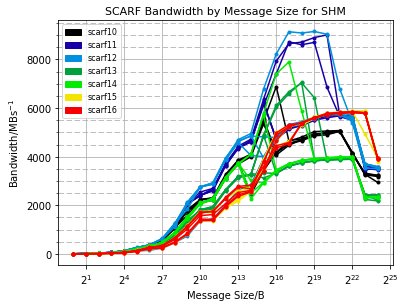
\includegraphics[width=\textwidth]{scarf_bandwidth-msgsize_shm}
                  \caption{SCARF}
                \end{subfigure}%
                \begin{subfigure}{.5\textwidth}
                  \centering
                  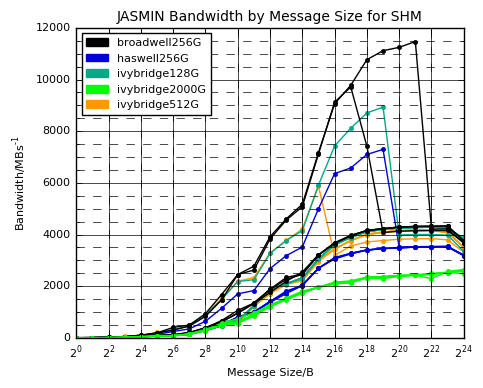
\includegraphics[width=\textwidth]{jasmin_bandwidth-msgsize_shm}
                  \caption{LOTUS}
                \end{subfigure}
            \caption{Before specifying CPUs}
            \label{figure:imb-before-cpus}
            \end{figure}

            \paragraph{}
            Figure \ref{figure:imb-before-cpus} shows the initial results for IMB over SCARF and LOTUS using SHM. Each colour represents a different host group and each line an individual repeat. For each host group, there are two distinct paths rather than one. For example, scarf11 has a bandwidth of roughly \SI{8300}{\mega\byte\per\second} for two repeats but roughly \SI{5200}{\mega\byte\per\second} for the other three at $2^{18}$\si{\byte}. Occasionally (as seen in scarf14 at $2^{17}$\si{\byte}) a repeat will begin on the higher path and drop down to the lower. A likely explanation is the multiple physical CPUs included in each host. The allocation is not set, allowing an SHM job to run with two processes on one CPU or with one process on each. It may be possible for a job to move from one CPU to two CPUs or vice versa which would lead to the switching behavior in Figure \ref{figure:imb-before-cpus}.

            \paragraph{}
            To eliminate this variation and to test if this is actually the cause, the tests were repeated over SHM for SCARF and LOTUS, specifically mapping to one or two CPUs. For one CPU, \mintinline{bash}{numactl --cpunodebind=0 --} was passed to \mintinline{bash}{mpirun} and \mintinline{bash}{-cpu_bind=MAP_CPU:0,15} for two. Figure \ref{figure:imb-after-cpus} shows the new results. The distinct paths in Figure \ref{figure:imb-before-cpus} are grouped by the CPU mapping and there is no longer a switch from one path to another.

            \begin{figure}[H]
                \centering
                \begin{subfigure}{.5\textwidth}
                  \centering
                  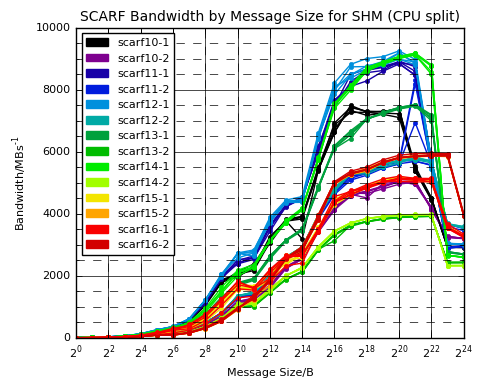
\includegraphics[width=\textwidth]{scarf_bandwidth-msgsize_shm_split}
                  \caption{SCARF}
                \end{subfigure}%
                \begin{subfigure}{.5\textwidth}
                  \centering
                  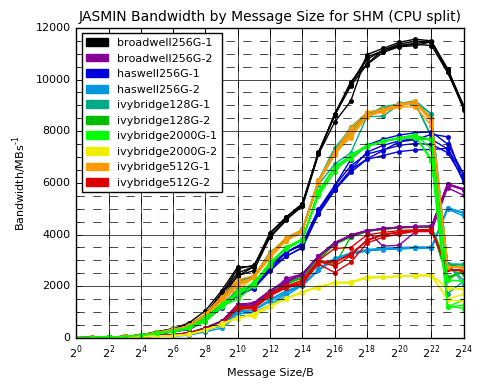
\includegraphics[width=\textwidth]{jasmin_bandwidth-msgsize_shm_split}
                  \caption{LOTUS}
                \end{subfigure}
            \caption{After specifying CPU mapping (given after the host group).}
            \label{figure:imb-after-cpus}
            \end{figure}

            \paragraph{} On the Cloud (Figure \ref{figure:imb-cloud-bandwidth-msgsize}) there is also a potential split between using one or two CPUs; the 11:25 and 13:05 runs on 2017-03-22 are considerably slower than the other runs. Unlike SCARF and LOTUS, there is no way to specify CPU mapping so this can't be tested further. The larger number of repeats should ensure results representative of normal Cloud usage.
            \begin{center}
                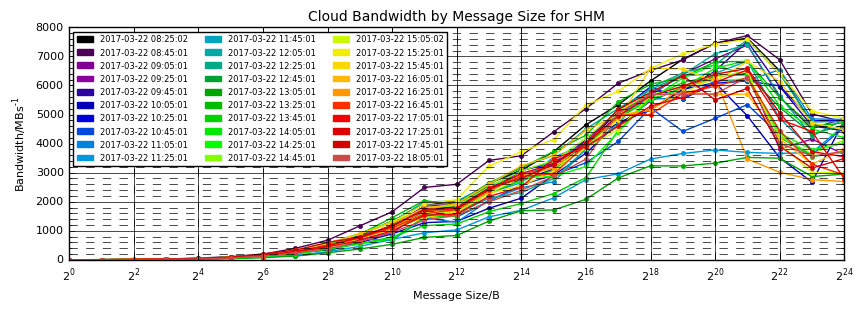
\includegraphics[width=\textwidth]{cloud_bandwidth-msgsize_shm}
                \captionsetup{type=figure}
                \caption{Cloud - unable to specify CPU mapping}
                \label{figure:imb-cloud-bandwidth-msgsize}
            \end{center}

        \subsubsection{Comparison of Latency}
            \label{analyse-results-imb-latency}

            \paragraph{}
            The results are compared by method of communication and then by improvements in hardware. The data (Appendix \ref{appendix:latency-data}) is presented as a log plot in Figure \ref{fig:compare_latency-hostgroup}.

            \begin{figure}[H]
                \centering
                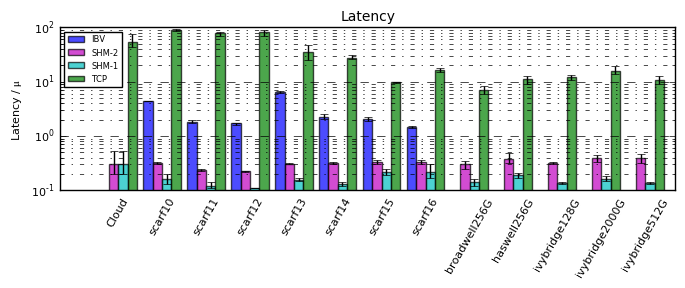
\includegraphics[width=\textwidth]{compare_latency-hostgroup}
                \caption{Comparison of latencies over different infrastructures and interconnects. The mean of the repeats for each combination is shown along with error bars for the range of repeats. After the adaptions in Section \ref{subsubsection:SHM-first-look}, SHM is split into SHM-1 and SHM-2 by the number of CPUs used. On the Cloud, there is no difference between these as the CPU mapping could not be specified and is unknown.}
                \label{fig:compare_latency-hostgroup}
            \end{figure}

            \paragraph{}
            Latency is mainly affected by the method of communication. Even ignoring the impact of host group, there is a clear ranking: SHM-1, SHM-2, IBV then TCP. As the processes span more interfaces - between nodes rather than within nodes - latency rises. SHM-1 has the lowest latency, perhaps taking advantage of a shared L3 cache and RAM - allowing each process to directly access the MPI shared buffer. With SHM-2, the distinct CPUs have separate L3 caches and rely on 'QuickPath Interconnect' to access memory allocated to the other processor [\cite{intel2009}]. Establishing the buffer over this additional protocol will add an extra overhead, explaining the greater latency. Similarly, inter-node communication over TCP/IBV adds another layer of protocols and hardware (e.g. switches, network cards), increasing the time to establish a connection. On SCARF (where direct comparison is possible) IBV is lower latency than TCP. This is also the case when comparing with LOTUS; SCARF's highest average latency for a host group over IBV (scarf13 at \SI{6.55}{\micro\second}) is smaller than LOTUS's lowest over TCP (broadwell256G at \SI{7.17}{\micro\second}).

            \paragraph{}
            The effect of newer hardware is less clear. Over TCP, SCARF latencies broadly reduce as hardware improves from scarf10 to scarf16. Certainly scarf15's \SI{9.70}{\micro\second} is better than \SI{89.49}{\micro\second} for scarf10. While there was a move from 1Gb to 10Gb Ethernet between scarf14 and scarf15, this can only be part of the explanation because scarf13 and scarf14 also show significantly lower latency than scarf10 with the same Ethernet hardware. The latency results for LOTUS do not depend as significantly on host group with all performing similarly although the newer Broadwell host group (\SI{7.17}{\micro\second}) is lower than the Haswell and Ivybridge host groups (11.05, 11.99 and 10.89 \si{\micro\second} respectively).

            \paragraph{}
            Despite improvements in hardware, the latency results for IBV and SHM remain mainly constant. Most IBV results are around \SI{2}{\micro\second} with scarf10 (\SI{4.38}{\micro\second}) slightly higher. This is perhaps due to older DDR Infiniband (although the similar upgrade from QDR to FDR after scarf14 did not have a noticeable effect). The results show better hardware having minimal effect on latency inside the node with all SCARF/LOTUS host groups at roughly \SI{0.15}{\micro\second} for SHM-1 and \SI{0.32}{\micro\second} for SHM-2.

            \paragraph{}
            The scarf13 IBV results are significantly higher than the others. To check for an error, the tests were additionally repeated ten times to check a wider variety of hosts but the new results agreed (mean latency \SI{6.36}{\micro\second}).

            \paragraph{}
            The Cloud manages to compete with some of the older SCARF hosts (10, 11, 12) over TCP. Without knowing the CPU mapping, it has similar results to the other systems (\SI{0.31}{\micro\second}) between two CPUs.

            \subsubsection{Comparison of Bandwidth}
            \label{analyse-results-imb-bandwidth}

            \paragraph{}
            The results for bandwidth are compared by method of communication and hardware. They are presented for three set message sizes and the maximum in Figure \ref{fig:compare_bandwidth-hostgroup_max} (data in Appendix \ref{appendix:bandwidth-data}). As the message size increases, the bandwidth increases because the constant setup time accounts for a smaller proportion of the total time taken.

            \paragraph{}
            Across these message sizes, the ranking is mainly the same as latency: SHM-1, SHM-2, IBV and then TCP. The reason is probably similar; the fastest data rates are achieved at close proximity to the CPU where data can be accessed over many lanes in parallel.

            \paragraph{}
            The benefit of improvements in hardware is clearer here than with latency. The TCP results for 10Gb Ethernet (scarf15, scarf16 and all of LOTUS) have roughly ten times the throughput as those with only 1Gb Ethernet. At max bandwidth, they both approach their specification (\SI{1250}{\mega\byte\per\second} / \SI{125}{\mega\byte\per\second}), indicating that they are a bottleneck. Over IBV, DDR on scarf10 is consistently the slowest. The benefit of FDR (used after scarf14) over QDR is clear when looking at the max bandwidth achieved (FDR greater than \SI{5500}{\mega\byte\per\second} with QDR less than \SI{3500}{\mega\byte\per\second}).

            \paragraph{}
            Across all message sizes, the SHM values are similar regardless of host group, suggesting that the newer hardware has not improved bandwidth for intra-node communication.

            \paragraph{}
            On scarf15/16, the max bandwidth results place IBV and SHM-2 slightly faster than SHM-1. For example, scarf15 had \SI{5145.80}{\mega\byte\per\second}, \SI{5876.91}{\mega\byte\per\second} and \SI{5670.07}{\mega\byte\per\second} for SHM-1, SHM-2, and IBV respectively. Comparing with the similar haswell256G hosts, it is SHM-1 (\SI{7683.80}{\mega\byte\per\second}) which stands out as the outlier. The explanation for this is an open question - the range of values over the repeats was small (\SI{51.39}{\mega\byte\per\second} for scarf15) and at least three different hosts were used suggesting that there is an underlying cause of this rather than a single error.

            \paragraph{}
            The Cloud outperforms the 1Gb Ethernet but cannot compete with 10Gb Ethernet or IBV. Ignoring scarf14 for the \SI{1024}{\byte} messages (where it came close), the Cloud had a significantly higher bandwidth than the 1Gb Ethernet hosts. For \SI{32768}{\byte} messages, \SI{184.26}{\mega\byte\per\second} is over three times as fast scarf14's \SI{56.77}{\mega\byte\per\second} but still slower than \SI{311.79}{\mega\byte\per\second} (the lowest result accross IBV and 10Gb Ethernet).

            \begin{figure}[H]
                \centering
                \begin{subfigure}{\textwidth}
                  \centering
                    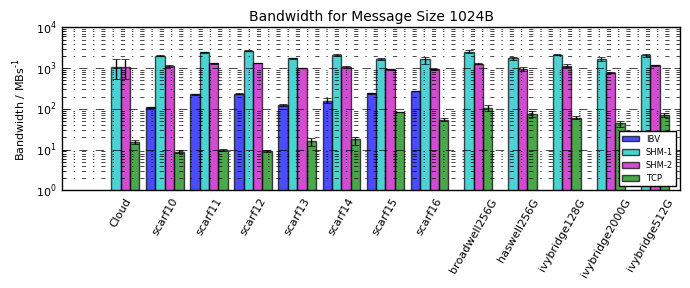
\includegraphics[width=\textwidth]{compare_bandwidth-hostgroup_1024}
                  \caption{1024\si{\byte} messages}
                \end{subfigure}

                \begin{subfigure}{\textwidth}
                  \centering
                     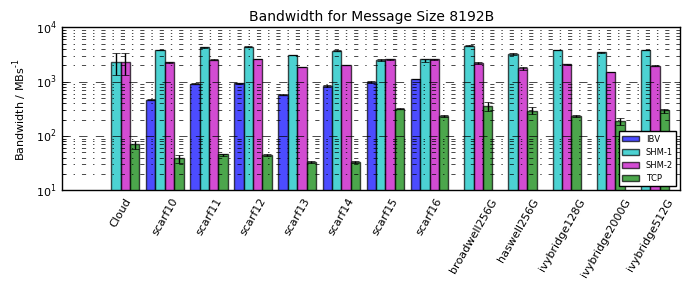
\includegraphics[width=\textwidth]{compare_bandwidth-hostgroup_8192}
                  \caption{8192\si{\byte} messages}
                \end{subfigure}
                %\caption{}
             \end{figure}

             \begin{figure}[H]\ContinuedFloat
                \centering
                \begin{subfigure}{\textwidth}
                  \centering
                    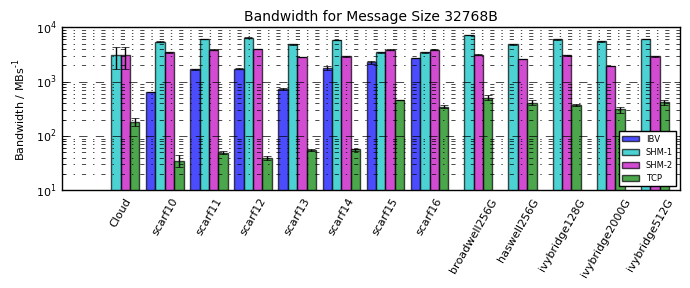
\includegraphics[width=\textwidth]{compare_bandwidth-hostgroup_32768}
                  \caption{32768\si{\byte} messages}
                \end{subfigure}

                \begin{subfigure}{\textwidth}
                  \centering
                    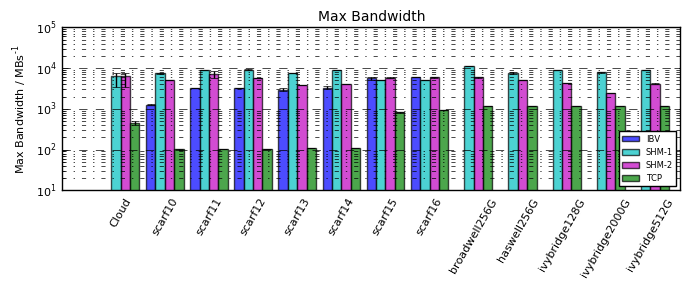
\includegraphics[width=\textwidth]{compare_bandwidth-hostgroup_max}

                  \caption{Max bandwidth over all message sizes}
                \end{subfigure}
                \caption{Comparison of bandwidths between host groups and protocols at different message sizes. Each bar shows the mean over the repeats with the range bars showing the range of repeats.}
                \label{fig:compare_bandwidth-hostgroup_max}
             \end{figure}

    \subsection{HPL}
        \begin{figure}
            \centering
            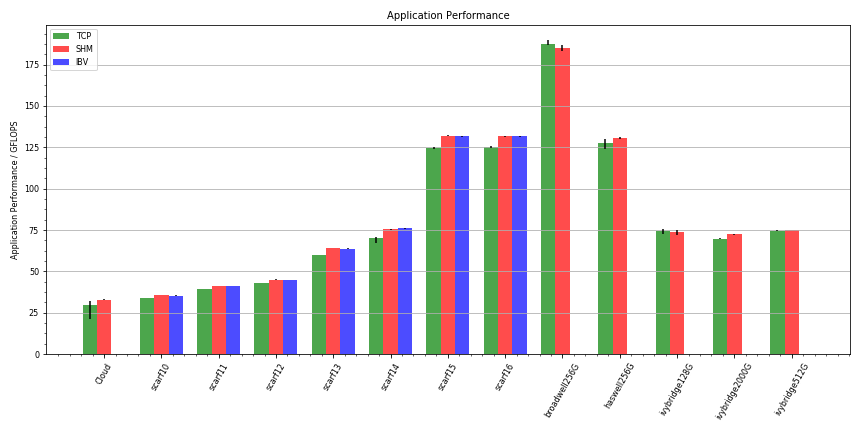
\includegraphics[width=\textwidth]{application_performance}
            \caption{Comparison of the application performance for different options as measured by HPL. The range over the repeats was small so after the initial IMB results, the experiment was not repeated splitting SHM-1 and SHM-2. The units are GFLOPS which refer to billion floating point operations per second.}
            \label{fig:application_performance}
        \end{figure}

        \paragraph{}
        The results for the HPL benchmarks are compared for the same choices. They are displayed in Figure \ref{fig:application_performance} from the data in Appendix \ref{appendix:hpl-data}.


        \paragraph{}
        As with latency and bandwidth, the same ranking broadly applies for application performance: SHM, IBV then TCP. Although the results are much closer, TCP is 4\% lower than SHM on average while IBV is 0.2\%. TCP performs much better on LOTUS than SCARF where results are comparable to SHM on all but the niche ivybridge2000G. The slightly lower FLOPS for inter-host communication is likely due to TCP and IBV's lower bandwidth and higher latency relative to SHM. Causing communications to take longer, this would have stalled the benchmark while it was waiting to transfer matrix elements.

        \paragraph{}
        Despite the interconnect ranking, Figure \ref{fig:application_performance} shows that to maximise application performance, choosing a faster CPU (e.g. Broadwell rather than Haswell) should be prioritised over interconnect as every TCP result is greater than the SHM results for the previous generations. There is a greater than linear increase in performance as the SCARF hardware iterates from 2010 to 2015/16 (roughly 35 to 130 GFLOPS). The results for LOTUS's Ivybridge and Haswell agree with their SCARF equivalents (scarf14 and scarf15/16 respectively) and the Broadwell host group achieves the highest results at over 185 GFLOPS for both TCP and SHM.

        \paragraph{}
        Although the results suggest that the Broadwell host group performed better over TCP than SHM, it is possible that the five SHM repeats were under representative. This could be the result of an external factor, perhaps interference from a busy host operating system. Given that the ranges do overlap, this is not a large cause for concern.

        \paragraph{}
        The Cloud was the worst performing in this test. With 33.01 GFLOPS over SHM, it was over 2 behind the next host group. As the other results have shown, this benchmark depends largely on CPU. One reason could be the virtualisation of CPUs which adds an additional overhead that is likely to slow the application down. Although the cloud allocates two virtual CPUs to a physical CPU, this would only throttle the application if more than half of the allocated virtual CPUs were active at a given time and there was competition for execution. From looking at monitoring, for at least some of the tests, there was not a high load on the hypervisor. Given that the range of results for SHM is low, I would suggest that this wasn't an issue for SHM. However, coupled with network interference from other users, this could be a reason for the large range of results for the Cloud over TCP.

\section{Conclusion}
    \paragraph{}
    Two benchmarks (IMB and HPL) were run over different options for SCARF, LOTUS and the Cloud to measure latency, bandwidth and parallel application performance. Both benchmarks were run between cores on the same host (initially over SHM) and between cores on separate hosts (using TCP and IBV on SCARF). The IMB results for SHM were later split into SHM-1 and SHM-2 spanning either one or two CPUs.

    \paragraph{}
    The results for all three benchmarks established the expected ranking between the methods of communication: SHM-1, SHM-2, IBV then TCP. This is in order of increasing latency or decreasing bandwidth and application performance. The difference in latency was orders of magnitude but particularly for larger message sizes and the latest version, IBV was comparable to SHM for bandwidth and application performance. Although the bandwidth for 10Gb Ethernet was reasonably far from SHM, it was also competitive when measuring application performance.

    \paragraph{}
    The impact of newer hardware on latency and bandwidth was varied. The move from 1Gb Ethernet to 10Gb Ethernet on SCARF reduced latency and increased bandwidth, especially on large message sizes. Similarly the move from DDR through QDR to FDR over IBV increased bandwidth. However this change didn't have a clear impact on latency. Also, newer processors did not seem to have a significant impact on latency or bandwidth over SHM-1 or SHM-2.

    \paragraph{}
    For application performance, newer processors were the key factor determining the results. However, it was notable that the inter-node communication (TCP on LOTUS and IBV on SCARF) achieved results similar to SHM which is promising for large scale parallel applications.

    \paragraph{}
    For bandwidth and latency, the Cloud performed close to SCARF and LOTUS over SHM (although closer to SHM-2 than SHM-1 without a CPU maping). Over TCP, it was competitive against SCARF's 1Gb Ethernet but was far behind TCP on LOTUS and IBV on SCARF. The parallel application performance was the lowest of all host groups, perhaps due to the virtualised CPUs.





\printbibliography[title={Sources}]



































\clearpage


\appendix
    \section*{Appendices}
    \addcontentsline{toc}{section}{Appendices}
    \renewcommand{\thesubsection}{\Alph{subsection}}

    \subsection{HPL SL6 Makefile}
    \label{appendix:makefile}

    \paragraph{}
    The comments are removed but the format follows the example in the \verb|hpl-2.2.tar| archive \verb|hpl-2.2/setup/Make.Linux_Intel64|. It should be saved as \verb|hpl-2.2/Make.Linux_SL6_Intel64|.
        \begin{code}
        \captionof{listing}{The HPL SL6 Makefile}
        \label{code:builds-cloud-make-linux_sl6_intel64}
        \begin{minted}{make}
SHELL        = /bin/sh
CD           = cd
CP           = cp
LN_S         = ln -fs
MKDIR        = mkdir -p
RM           = /bin/rm -f
TOUCH        = touch
ARCH         = Linux_SL6_Intel64
TOPdir       = $(HOME)/hpl-2.2
INCdir       = $(TOPdir)/include
BINdir       = $(TOPdir)/bin/$(ARCH)
LIBdir       = $(TOPdir)/lib/$(ARCH)
HPLlib       = $(LIBdir)/libhpl.a
MPdir        = /usr
MPinc        = -I$(MPdir)/include/openmpi-1.10-x86_64
MPlib        = $(MPdir)/lib64/openmpi-1.10/lib/libmpi.so
LAinc        =  /usr/include/openblas/
LAlib        =  /usr/lib64/libopenblas.so
F2CDEFS      = -DAdd__ -DF77_INTEGER=int -DStringSunStyle
HPL_INCLUDES = -I$(INCdir) -I$(INCdir)/$(ARCH) -I$(LAinc) $(MPinc)
HPL_LIBS     = $(HPLlib) $(LAlib) $(MPlib)
HPL_OPTS     = -DHPL_DETAILED_TIMING -DHPL_PROGRESS_REPORT
HPL_DEFS     = $(F2CDEFS) $(HPL_OPTS) $(HPL_INCLUDES)
CC           = mpicc
CCNOOPT      = $(HPL_DEFS)
OMP_DEFS     = -openmp
CCFLAGS      = $(HPL_DEFS) -O3 -w -z noexecstack -z relro -z now -Wall
LINKER       = $(CC)
LINKFLAGS    = $(CCFLAGS) $(OMP_DEFS) -mt_mpi
ARCHIVER     = ar
ARFLAGS      = r
RANLIB       = echo

        \end{minted}
        \end{code}

    \clearpage

    \subsection{IMB Example Output}
        \label{appendix:imb-example-output}

        \begin{minted}{text}
#---------------------------------------------------
# Benchmarking PingPong
# #processes = 2
#---------------------------------------------------
       #bytes #repetitions      t[usec]   Mbytes/sec
            0         1000         0.24         0.00
            1         1000         0.31         3.03
            2         1000         0.33         5.73
            4         1000         0.32        12.02
            8         1000         0.33        23.29
           16         1000         0.36        42.87
           32         1000         0.32        95.24
           64         1000         0.34       177.65
          128         1000         0.38       322.93
          256         1000         0.47       524.46
          512         1000         0.57       853.69
         1024         1000         0.73      1334.20
         2048         1000         1.02      1916.71
         4096         1000         2.00      1957.00
         8192         1000         2.97      2629.12
        16384         1000         5.06      3086.37
        32768         1000         8.39      3723.58
        65536         1000        13.45      4648.40
       131072         1000        23.42      5338.11
       262144         1000        40.61      6155.58
       524288         1000        72.47      6899.88
      1048576         1000       134.10      7456.95
      2097152         1000       262.16      7628.87
      4194304         1000       614.76      6506.58
      8388608         1000      1714.74      4665.43
     16777216         1000      3617.98      4422.35
        \end{minted}

    \clearpage

    \subsection{HPL Configuration File}
        \label{appendix:hpl-conf}

        \begin{minted}{text}
The HPL Configuration File for comparing LOTUS, SCARF
and the Cloud in SCD.
not_used     output file name (if any)
6            device out (6=stdout,7=stderr,file)
1            # of problems sizes (N)
44640        Ns
1            # of NBs
180          NBs
0            PMAP process mapping (0=Row-,1=Column-major)
1            # of process grids (P x Q)
2            Ps
2            Qs
16.0         threshold
1            # of panel fact
1            PFACTs (0=left, 1=Crout, 2=Right)
1            # of recursive stopping criterium
4            NBMINs (>= 1)
1            # of panels in recursion
2            NDIVs
1            # of recursive panel fact.
2            RFACTs (0=left, 1=Crout, 2=Right)
1            # of broadcast
1            BCASTs (0=1rg,1=1rM,2=2rg,3=2rM,4=Lng,5=LnM)
1            # of lookahead depth
1            DEPTHs (>=0)
2            SWAP (0=bin-exch,1=long,2=mix)
180          swapping threshold
0            L1 in (0=transposed,1=no-transposed) form
0            U  in (0=transposed,1=no-transposed) form
1            Equilibration (0=no,1=yes)
8            memory alignment in double (> 0)
        \end{minted}

    \clearpage

    \subsection{HPL Example Output}
        \label{appendix:hpl-example-output}


        \begin{minted}{text}
================================================================================
HPLinpack 2.2  --  High-Performance Linpack benchmark  --   February 24, 2016
Written by A. Petitet and R. Clint Whaley,  Innovative Computing Laboratory, UTK
Modified by Piotr Luszczek, Innovative Computing Laboratory, UTK
Modified by Julien Langou, University of Colorado Denver
================================================================================
...
--------------------------------------------------------------------------------

- The matrix A is randomly generated for each test.
- The following scaled residual check will be computed:
      ||Ax-b||_oo / ( eps * ( || x ||_oo * || A ||_oo + || b ||_oo ) * N )
- The relative machine precision (eps) is taken to be               1.110223e-16
- Computational tests pass if scaled residuals are less than                16.0

Column=000000180 Fraction= 0.4% Gflops=5.839e+03
Column=000000360 Fraction= 0.8% Gflops=6.953e+01
Column=000000540 Fraction= 1.2% Gflops=5.027e+01
...
Column=000044460 Fraction=99.6% Gflops=3.297e+01
================================================================================
T/V                N    NB     P     Q               Time                 Gflops
--------------------------------------------------------------------------------
WR11R2C4       44640   180     2     2            1799.04              3.297e+01
HPL_pdgesv() start time Sun Mar 26 23:50:20 2017

HPL_pdgesv() end time   Mon Mar 27 00:20:19 2017

--VVV--VVV--VVV--VVV--VVV--VVV--VVV--VVV--VVV--VVV--VVV--VVV--VVV--VVV--VVV-
Max aggregated wall time rfact . . . :               6.76
+ Max aggregated wall time pfact . . :               1.22
+ Max aggregated wall time mxswp . . :               0.62
Max aggregated wall time update  . . :            1792.06
+ Max aggregated wall time laswp . . :              49.64
Max aggregated wall time up tr sv  . :               0.36
--------------------------------------------------------------------------------
||Ax-b||_oo/(eps*(||A||_oo*||x||_oo+||b||_oo)*N)=        0.0006845 ...... PASSED
================================================================================

Finished      1 tests with the following results:
              1 tests completed and passed residual checks,
              0 tests completed and failed residual checks,
              0 tests skipped because of illegal input values.
--------------------------------------------------------------------------------

End of Tests.
================================================================================

        \end{minted}
    \subsection{Latency Data}
        \label{appendix:latency-data}

        \begin{center}
            \centering
            \begin{tabular}{ |c||c|c|c|c|  }
             \hline
             \multirow{2}{*}{Host group} & \multicolumn{4}{c|}{Mean latency / \si{\micro\second}} \\
             \cline{2-5}
                                      & SHM-1 & SHM-2 & TCP & IBV\\
             \hline
                Cloud & \multicolumn{2}{c|}{0.31} & 54.74 & n/a\\
                scarf10 & 0.16 & 0.32 & 89.49 & 4.38\\
                scarf11 & 0.12 & 0.24 & 77.21 & 1.83\\
                scarf12 & 0.11 & 0.23 & 83.53 & 1.71\\
                scarf13 & 0.16 & 0.31 & 35.22 & 6.55\\
                scarf14 & 0.13 & 0.32 & 26.93 & 2.22\\
                scarf15 & 0.21 & 0.34 & 9.70 & 2.02\\
                scarf16 & 0.22 & 0.34 & 16.44 & 1.47\\
                broadwell256G & 0.14 & 0.30 & 7.17 & n/a\\
                haswell256G & 0.19 & 0.37 & 11.05 & n/a\\
                ivybridge128G & 0.13 & 0.32 & 11.99 & n/a\\
                ivybridge2000G & 0.16 & 0.39 & 15.90 & n/a\\
                ivybridge512G & 0.13 & 0.40 & 10.89 & n/a\\

             \hline
            \end{tabular}
            \captionsetup{type=table}
            \caption{The mean latency over all repeats, split by host group as shown in Figure \ref{fig:compare_latency-hostgroup}}
        \end{center}






    \subsection{Bandwidth Data}
        \label{appendix:bandwidth-data}

        The following data is for the four charts in Figure \ref{fig:compare_bandwidth-hostgroup_max}.

        \begin{center}
            \centering
            \begin{tabular}{ |c||c|c|c|c|  }
             \hline
             \multirow{2}{*}{Host group} & \multicolumn{4}{c|}{Mean bandwidth of 1024B messages / \si{\mega\byte\per\second}} \\
             \cline{2-5}
                                      & SHM-1 & SHM-2 & TCP & IBV\\
             \hline
                Cloud & \multicolumn{2}{c|}{1086.01} & 15.58 & n/a\\
                scarf10 & 2035.05 & 1132.61 & 8.90 & 109.43\\
                scarf11 & 2443.99 & 1318.35 & 9.63 & 225.26\\
                scarf12 & 2694.70 & 1355.99 & 9.30 & 234.97\\
                scarf13 & 1739.76 & 995.17 & 16.31 & 123.09\\
                scarf14 & 2103.48 & 1058.89 & 17.76 & 154.32\\
                scarf15 & 1659.08 & 927.46 & 83.44 & 243.07\\
                scarf16 & 1644.23 & 942.36 & 53.18 & 278.32\\
                broadwell256G & 2547.62 & 1263.69 & 102.12 & n/a\\
                haswell256G & 1724.22 & 975.50 & 73.79 & n/a\\
                ivybridge128G & 2121.81 & 1127.32 & 60.85 & n/a\\
                ivybridge2000G & 1695.40 & 775.68 & 44.79 & n/a\\
                ivybridge512G & 2065.02 & 1167.25 & 69.32 & n/a\\
             \hline
            \end{tabular}
            \captionsetup{type=table}
            \caption{The mean bandwidth for the 1024B messages split by host group}
        \end{center}

         \begin{center}
            \centering
            \begin{tabular}{ |c||c|c|c|c|  }
             \hline
             \multirow{2}{*}{Host group} & \multicolumn{4}{c|}{Mean bandwidth of 8192B messages / \si{\mega\byte\per\second}} \\
             \cline{2-5}
                                      & SHM-1 & SHM-2 & TCP & IBV\\
             \hline
                Cloud & \multicolumn{2}{c|}{2331.78} & 70.82 & n/a\\
                scarf10 & 3786.75 & 2269.98 & 39.92 & 468.49\\
                scarf11 & 4266.71 & 2559.63 & 45.96 & 913.84\\
                scarf12 & 4399.96 & 2601.34 & 45.63 & 935.66\\
                scarf13 & 3153.47 & 1891.89 & 32.81 & 579.11\\
                scarf14 & 3735.09 & 2005.55 & 33.34 & 822.42\\
                scarf15 & 2513.02 & 2563.46 & 318.38 & 988.26\\
                scarf16 & 2566.26 & 2568.84 & 233.96 & 1122.51\\
                broadwell256G & 4615.70 & 2204.37 & 352.73 & n/a\\
                haswell256G & 3248.41 & 1752.09 & 289.13 & n/a\\
                ivybridge128G & 3794.90 & 2106.11 & 235.51 & n/a\\
                ivybridge2000G & 3479.32 & 1514.62 & 188.94 & n/a\\
                ivybridge512G & 3785.00 & 1983.11 & 295.25 & n/a\\
             \hline
            \end{tabular}
            \captionsetup{type=table}
            \caption{The mean bandwidth for the 8192B messages split by host group}
        \end{center}

         \begin{center}
            \centering
            \begin{tabular}{ |c||c|c|c|c|  }
             \hline
             \multirow{2}{*}{Host group} & \multicolumn{4}{c|}{Mean bandwidth of 32768B messages/ \si{\mega\byte\per\second}} \\
             \cline{2-5}
                                      & SHM-1 & SHM-2 & TCP & IBV\\
             \hline
                Cloud & \multicolumn{2}{c|}{3164.26} & 184.26 & n/a\\
                scarf10 & 5432.64 & 3478.14 & 34.99 & 654.38\\
                scarf11 & 6071.52 & 3879.78 & 48.05 & 1699.70\\
                scarf12 & 6503.35 & 3952.47 & 40.03 & 1743.98\\
                scarf13 & 4855.00 & 2841.63 & 55.67 & 747.12\\
                scarf14 & 5775.77 & 2931.54 & 56.77 & 1796.93\\
                scarf15 & 3486.68 & 3905.40 & 463.96 & 2308.61\\
                scarf16 & 3473.62 & 3881.20 & 342.79 & 2702.85\\
                broadwell256G & 7150.79 & 3160.15 & 502.72 & n/a\\
                haswell256G & 4872.27 & 2633.92 & 409.64 & n/a\\
                ivybridge128G & 6045.88 & 3041.11 & 371.36 & n/a\\
                ivybridge2000G & 5605.09 & 1968.71 & 311.79 & n/a\\
                ivybridge512G & 6033.94 & 2946.58 & 429.37 & n/a\\
             \hline
            \end{tabular}
            \captionsetup{type=table}
            \caption{The mean bandwidth for the 32768B messages split by host group}
        \end{center}

         \begin{center}
            \centering
            \begin{tabular}{ |c||c|c|c|c|  }
             \hline
             \multirow{2}{*}{Host group} & \multicolumn{4}{c|}{Mean of max bandwidths / \si{\mega\byte\per\second}} \\
             \cline{2-5}
                                      & SHM-1 & SHM-2 & TCP & IBV\\
             \hline
                Cloud & \multicolumn{2}{c|}{6504.27} & 456.42 & n/a\\
                scarf10 & 7419.95 & 5048.19 & 101.54 & 1270.66\\
                scarf11 & 8877.11 & 6974.27 & 103.09 & 3215.99\\
                scarf12 & 9121.70 & 5787.32 & 102.91 & 3207.53\\
                scarf13 & 7504.84 & 3927.28 & 110.51 & 2940.26\\
                scarf14 & 9153.45 & 3973.65 & 111.81 & 3267.56\\
                scarf15 & 5145.80 & 5876.91 & 825.88 & 5670.07\\
                scarf16 & 5140.57 & 5905.49 & 934.16 & 5975.28\\
                broadwell256G & 11468.01 & 5920.18 & 1174.91 & n/a\\
                haswell256G & 7683.80 & 5006.57 & 1171.09 & n/a\\
                ivybridge128G & 9115.23 & 4299.59 & 1172.70 & n/a\\
                ivybridge2000G & 7808.32 & 2417.75 & 1163.62 & n/a\\
                ivybridge512G & 9082.18 & 4167.02 & 1172.76 & n/a\\

             \hline
            \end{tabular}
            \captionsetup{type=table}
            \caption{The mean of the max bandwidth over all message sizes for each host group }
        \end{center}

    \subsection{HPL Results}
        \label{appendix:hpl-data}
        \begin{center}
            \centering
            \begin{tabular}{ |c||c|c|c|  }
             \hline
             \multirow{2}{*}{Host group} & \multicolumn{3}{c|}{Application Performance / GFLOPS} \\
             \cline{2-4}
                                      & SHM & TCP & IBV\\
             \hline
                  Cloud & 33.01 & 29.66 & n/a\\
                  scarf10 & 35.62 & 34.07 & 35.42\\
                  scarf11 & 41.31 & 39.37 & 41.14\\
                  scarf12 & 45.06 & 42.79 & 44.94\\
                  scarf13 & 64.09 & 59.77 & 63.77\\
                  scarf14 & 75.64 & 70.10 & 75.98\\
                  scarf15 & 132.06 & 124.66 & 131.66\\
                  scarf16 & 131.64 & 125.24 & 131.60\\
                  broadwell256G & 185.32 & 187.62 & n/a\\
                  haswell256G & 130.50 & 127.54 & n/a\\
                  ivybridge128G & 73.98 & 74.72 & n/a\\
                  ivybridge2000G & 72.57 & 69.81 & n/a\\
                  ivybridge512G & 74.96 & 74.61 & n/a\\
             \hline
            \end{tabular}
            \captionsetup{type=table}
            \caption{The application performance as measured by HPL for the different options}
        \end{center}

\end{document}
